\chapter{System architecture}
The library is based on the client-server architectural pattern and is indeed split in two main modules: 
\begin{itemize}
	\item[Client module] Provide the main functionalities to connect and communicate with a game server. In particular allows the client side developer to create rooms (that will be hosted on the server) and to perform operations on them (e.g join, leave, message...).
	\item[Server module] Internally implements the logic to handle client connections and allows the developer to run a gameserver and define new type of rooms.
\end{itemize}

Cient and server however are not fully separated; they share some common concepts among which the most important, as emerged from the requirements, is the concept of Room.

\section{Room}
\begin{figure}[H]
	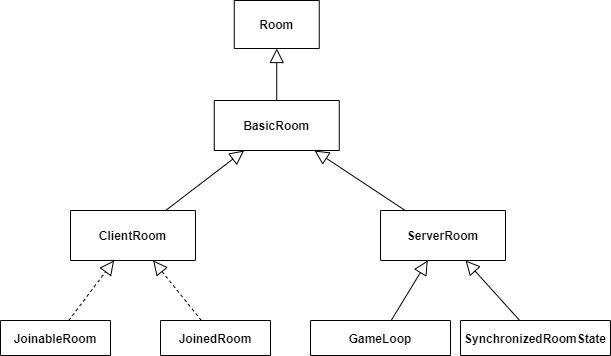
\includegraphics[scale=0.7]{images/3-architecture/room-class.png}
	\caption{Room design class diagram}
	\label{fig:room_classes}
\end{figure}

A room, at the most abstract level, is an entity wih a unique id and some shared properties. This fields are visible both on the client and the server. Then each module extends his own concept of room. 

\bigskip
\textit{ServerRoom}
\\
The server room is the one that will be used by the server side developer. It aggregates a list of client and provides the main methods to communicate with them (i.e. tell and broadcast).  This class is meant to be abstract so that the user can extend it and define his own behavior (as expressed in requirement 2.1 of table \ref{table:server-f-req})). Since the developer may want to automatically synchronize the state of the game and have an inner game loop (requirements 2.1.2.1 and 2.1.2.2), there are two extension of the server room: SynchronizedState and GameLoop that provide this functionalities.

\bigskip
\textit{ClientRoom}
\\
This is, on the other hand, the room that a client side developer will use. The user can retrieve a list of JoinableRoom from the server; these expose the method \textit{join} that sends a request to the game server to join the given room; a JoinableRoom can also be used to reconnect to a previously left room as express in requirement 5 of Table \ref{table:client-f-req}. Once the joining process to a specific room succedes, a JoinedRoom is created and the user can use it to perform operation on the room (requirements 4, 7, 8 of table \ref{table:client-f-req} ) 

\section{Server architecture}
The main components of the server side architecture are visible in figure \ref{fig:server_classes}. 

\begin{figure}[H]
	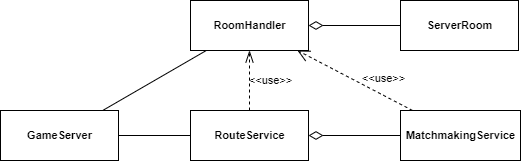
\includegraphics[scale=0.7]{images/3-architecture/server_architecture-classes.png}
	\caption{Server architecture class diagram}
	\label{fig:server_classes}
\end{figure}

\bigskip
\textit{GameServer}
\\
The GameServer is a facade component that is exposed to the user and provides the functionalities to: start and terminate a gameserver; define new type of rooms; create public rooms. To do so, it internally creates two other components that are the RouteService and the RoomHandler.

\bigskip
\textit{RoomHandler}
\\
As the name suggests, the RoomHandler is the handler of the rooms in the application. The purpose of this componenet is to provide functionalities concerning rooms, in particular:
\begin{itemize}
	\item get the list of available rooms
	\item define new type of rooms
	\item create rooms (with and without matchmaking)
	\item query rooms by their properties
	\item connect clients to a specific room
\end{itemize}

\bigskip
\textit{RouteService}
\\
The RouteService defines the routes that the server will listen on and implements all the handlers associated with them. Some routes are fixed since they are used by the library itself and are descibed in table \ref{table:server_routes}; 


\begin{table}[H]
	\begin{tabular}{p{2cm}p{4cm}p{2cm}p{5.5cm}}
		\textbf{Http Method} & \textbf{Path}	  & \textbf{Payload}  & \textbf{Result}                                                            		\\\\
		GET                  & /rooms             & filters           & get all the rooms that match the filters in the payload                        	\\\\
		GET                  & /rooms/:id         & empty             & get the room with the given id                                                 	\\\\
		GET                  & /rooms/:type       & filters           & get all the rooms with the given type (filtered by filters in the payload)     	\\\\
		GET                  & /rooms/:type/:id   & empty             & get the room with the given id searching among rooms of the given type         	\\\\
		POST                 & /rooms/:type       & options           & create a room of the given type with the option passed in the payload          	\\\\
		GET                  & /connection/:id    & websocket request & open a web socket connection with the room that has the given id               	\\\\
		GET                  & /matchmaking/:type & websocket request & open a web socket with the matchmaking service relative to the given room type 	\\\\
	\end{tabular}
	\caption{\label{table:server_routes} \textit{Server basic routes}}
\end{table}

All the routes that requires to perform operation on rooms are managed by the RoomHandler, while routes concerning matchmaking are managed by the appropriate MatchmakingService.


\bigskip
\textit{MatchmakingService}
\\
A MatchmakingService is a component that implements the matchmaking logic expressed in section \ref{server-requirements-gathering} for a given type of room. It use a strategy defined by the user to create client groups and uses a RoomHandler to create the room that will host the match.


\section{Client Architecture}

\section{Client-Server Interaction}
\subsection{Websockets}








